\chapter{Mengenal Kecerdasan Buatan dan Scikit-Learn}

\section{Teori}
Praktek teori penunjang yang dikerjakan :
\begin{enumerate}
\item
Definisi, Sejarah dan perkembangan Kecerdasan Buatan \textit{Artifical Intelligence}. \textit{Artifical Intelligence} merupakan ilmu yang ada pada bidang komputer yang memungkinkan untuk suatu sistem agar dapat menyelesaikan permasalahan.\\
Pada akhir tahun 1955 AI pertama muncul berkat Newell dan Simon dengan adanya perkembangan perkembangan \textit{The Logic Theorist} .Pada 1956, istilah AI pertama kali diciptakan di Darmouth College ketika menyelengarakan konferensi dengan nama \textit{The Dartmouth summer research project on artificial intelligence}. konferensi tersebut diselengarakan untuk memancing.

\item
Definisi supervised learning, klasifikasi, regresi dan unsupervised learning. Data set, training set dan testing set.
\begin{itemize}

	\item Supervised Learning
    \par
    \textit{Supervised Learning} sebuah pembelajaran yang ditentukan berdasarkan penggunaan traning set yang berlabel.

    \item Klasifikasi
    \par
    Klasifikasi adalah mengidentifikasi suatu data menjadi sebuah bagian dari kelas berdasarkan label.

	\item Regresi
	\par 
	Regresi adalah mendefinisikan relasi antara dua variable maupun lebih seperti variable terikat dan variabel bebas untuk melihat selisih nilai prediksi dengan nilai real.

    \item Data set, Training set dan Testing set
    \par
    Data set adalah kumpulan data. Kemudian training set adalah  data set yang berfungsi melatih suatu algoritma untuk mencapai suatu tujuan, dan testing set yaitu data set yang digunakan untuk mengetahui akurasi dari algoritma yang sudah di latih sebelumnya.

	\item Unsupervised Learning
	\par
	\textit{Unsupervised Learning} sebuah pembelajaran yang ditentukan berdasarkan penggunaan traning set yang tidak berlabel. 

\end{itemize}
\end{enumerate}

\section{Instalasi}
\begin{enumerate}
\item
Pertama lakukan instalasi anaconda navigator agar bisa mengakses spyder untuk mengeksekusi scikit-learn pada link dibawah.\\
gunakan "https://docs.anaconda.com/anaconda/install/windows/"\\
https://youtu.be/CXhTCjNudAA

\begin{figure}[!htbp]
    \centering
    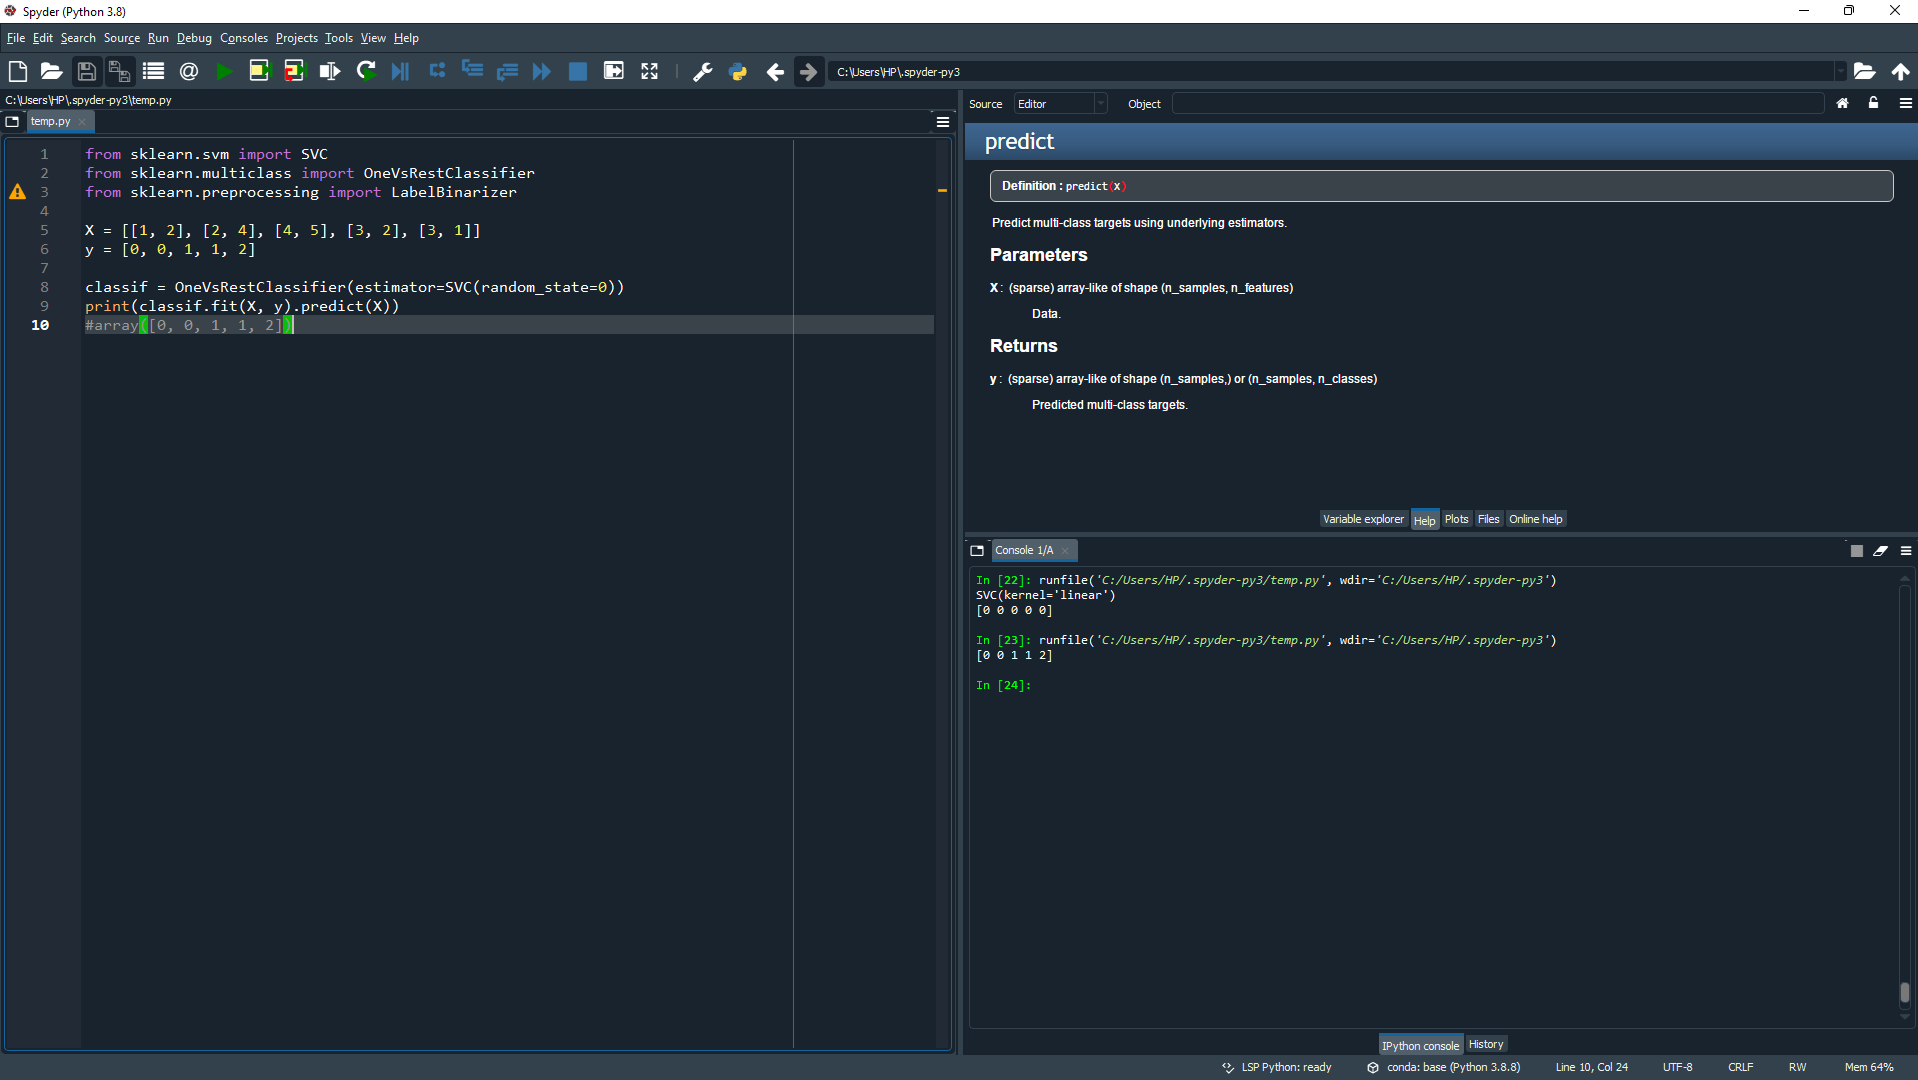
\includegraphics[scale=0.4]{figures/5.png}
    \end{figure}

\item
Mencoba Loading an example dataset, menjelaskan maksud dari tulisan tersebut dan mengartikan per baris
\begin{figure}[!htbp]
    \centering
    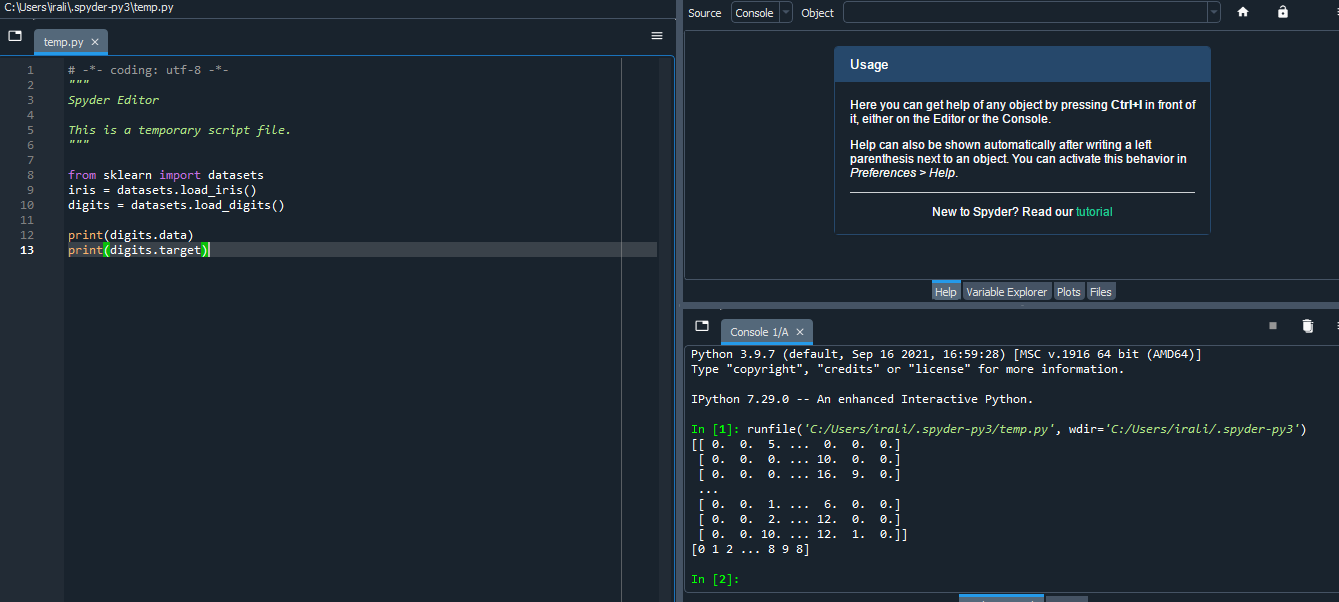
\includegraphics[scale=0.4]{figures/2.png}
    \end{figure}

\newpage
\item
Mencoba Learning and predicting, menjelaskan maksud dari tulisan tersebut dan mengartikan per baris
\begin{figure}[!htbp]
    \centering
    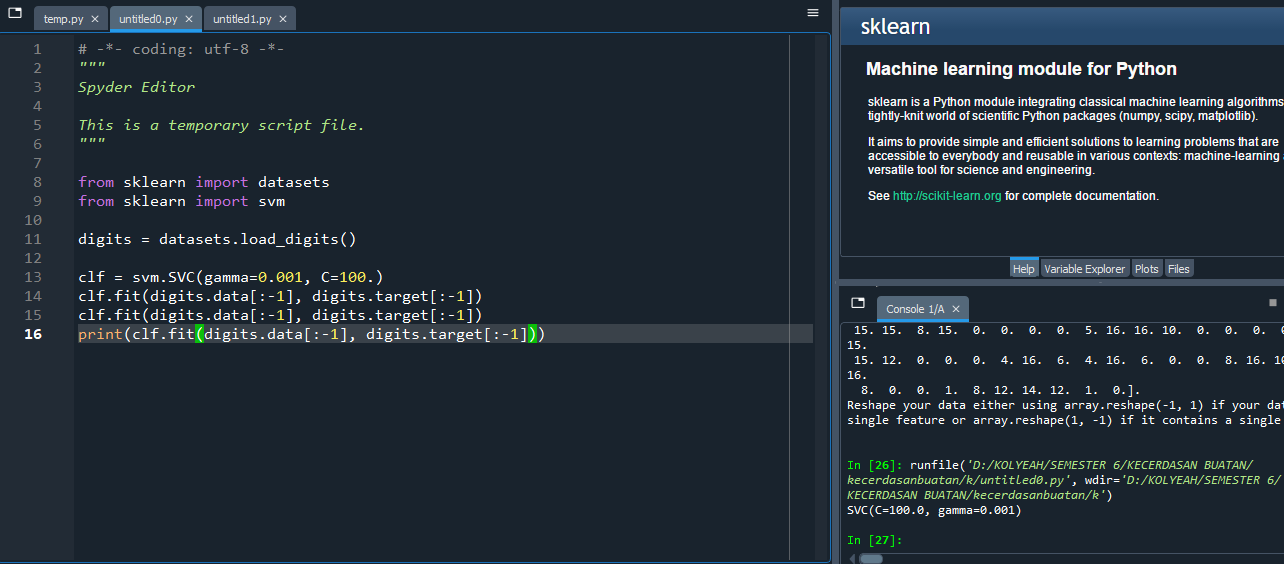
\includegraphics[scale=0.4]{figures/3.png}
    \end{figure}


\item
Mencoba Model persistence, menjelaskan maksud dari tulisan tersebut dan mengartikan per baris. menggunakan 2 cara yaitu menggunakan pickle atau menggunakan joblib
\begin{figure}[!htbp]
    \centering
    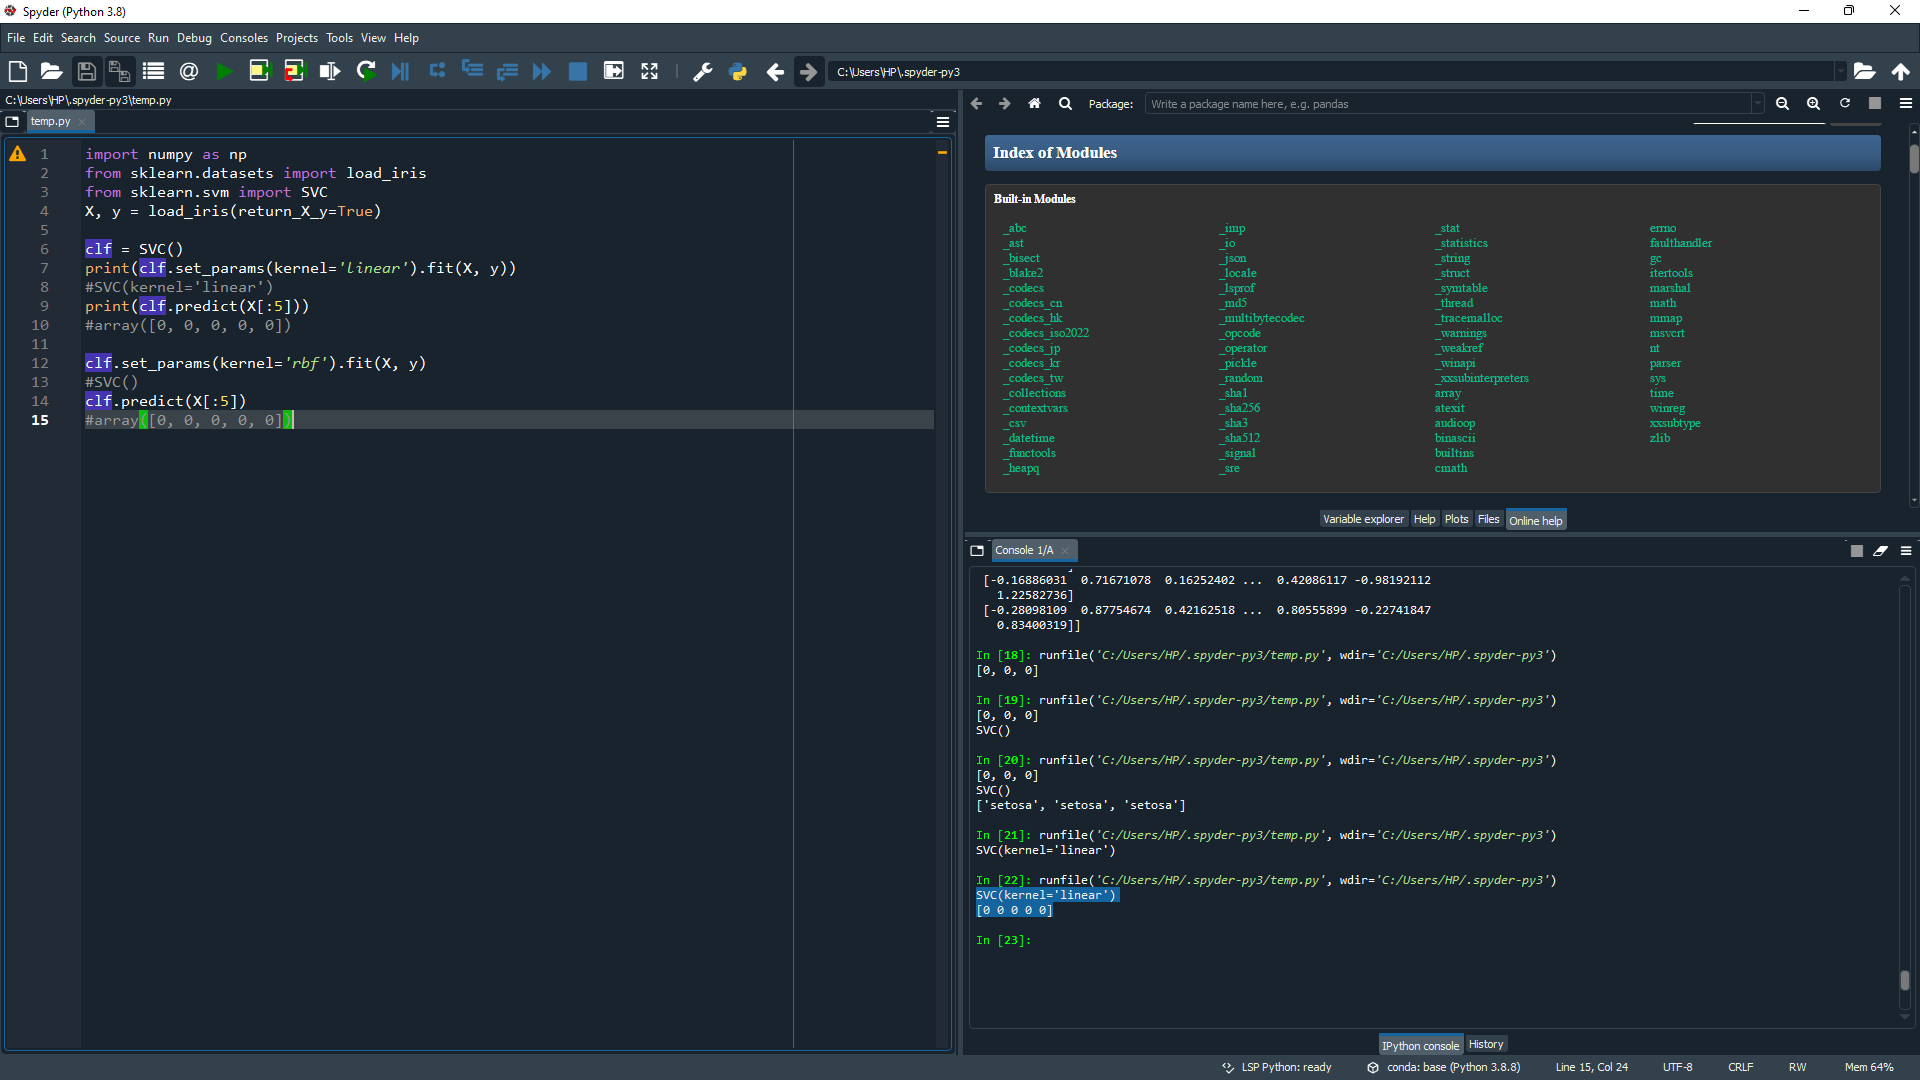
\includegraphics[scale=0.4]{figures/4.png}\\
    \end{figure}

\newpage
\begin{figure}[!htbp]
    \centering
    \end{figure}


\item 
Mencoba Conventions, menjelaskan maksud dari tulisan tersebut dan mengartikan per baris 
\begin{lstlisting}[language=Python]
import numpy as np  #library
from sklearn import random_projection, svm, datasets 
from sklearn.datasets import load_iris
from sklearn.multiclass import OneVsRestClassifier
from sklearn.preprocessing import LabelBinarizer
from sklearn.preprocessing import MultiLabelBinarizer
from sklearn.svm import SVC

iris = datasets.load_iris()


#Type Casting
rng = np.random.RandomState(0) 
X = rng.rand(10, 2000) 
X = np.array(X, dtype='float32')
print(X.dtype)

transformer = random_projection.GaussianRandomProjection()
X = transformer.fit_transform(X)
print(X.dtype)

clf = svm.SVC()
clf.fit(iris.data, iris.target)
print(clf.fit(iris.data, iris.target))

list(clf.predict(iris.data[:3]))

print((clf.predict(iris.data[:3])))

clf.fit(iris.data, iris.target_names[iris.target])
print(clf.fit(iris.data, iris.target_names[iris.target]))

list(clf.predict(iris.data[:3]))
print(list(clf.predict(iris.data[:3])))

#refitting and updating paramater
X, y = load_iris(return_X_y=True)
clf = svm.SVC()

clf.set_params(kernel='linear').fit(X, y)
print(clf.set_params(kernel='linear').fit(X, y))

clf.predict(X[:5])
print(clf.predict(X[:5]))

#Multiclass vs multilabel fitting
X = [[1, 2], [2, 4], [4, 5], [3, 2], [3, 1]]
y = [0, 0, 1, 1, 2]

classif = OneVsRestClassifier(estimator=SVC(random_state=0))
classif.fit(X, y).predict(X)
print(classif.fit(X, y).predict(X))

y = LabelBinarizer().fit_transform(y)
classif.fit(X, y).predict(X)
print(classif.fit(X, y).predict(X))

y = y = [[0, 1], [0, 2], [1, 3], [0, 2, 3], [2, 4]]
y = MultiLabelBinarizer().fit_transform(y)
print(classif.fit(X, y).predict(X))
\end{lstlisting}
\end{enumerate}



\section{Penanganan Error}
Dari percobaan yang dilakukan di atas, apabila mendapatkan error maka:

\begin{enumerate}
	\item
	skrinsut error\
    \begin{figure}[!htbp]
        \centering
        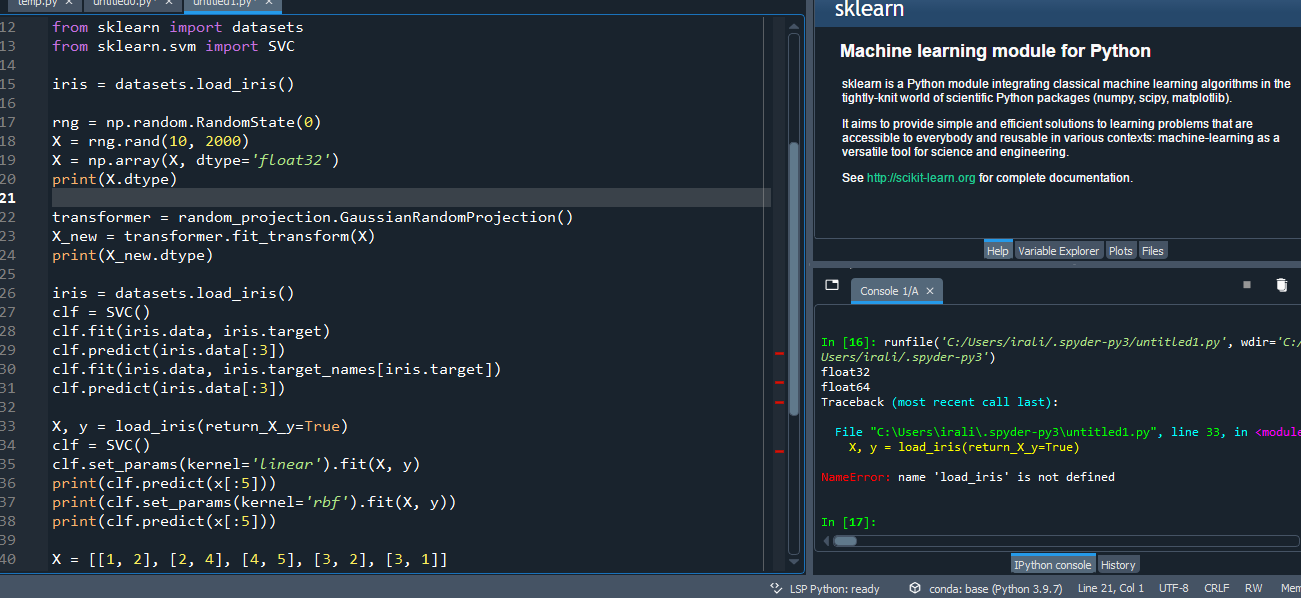
\includegraphics[scale=0.5]{figures/6.png}
        \end{figure}

	\item
Tuliskan kode eror dan jenis errornya\
    \begin{enumerate}
        \item invalid syntax
    \end{enumerate}

	\item
Solusi pemecahan masalah error tersebut\
\begin{enumerate}
    \item Lakukan pengecekan kembali terhadap kode, karena bisa saja ada titik koma yang terlewat.
    \begin{figure}[!htbp]
        \centering
        \end{figure}
    
\end{enumerate}

\end{enumerate}

